% Dieses Kapitel bildet zusammen mit dem folgenden Kapitel Diskussion den Hauptteil der Arbeit. In übersichtlicher Gliederung und sinnvoller Reihenfolge wird dargestellt, was mittels der eingesetzten Methodik im Hinblick auf die Zielsetzung herausgefunden werden konnte. Die Strukturierung des Kapitels orientiert sich an der Theorie und Methodik. Mit Hilfe von Grafiken und Diagrammen (siehe 2.8.4) werden die Ergebnisse wertfrei dargestellt. Eine Interpretation erfolgt an dieser Stelle noch nicht.
\chapter{Ergebnisse}
	Das auf Basis der vorangegangenen Überlegungen entwickelte Gerät soll im folgenden anhand gerenderter Darstellungen näher erläutert werden.
	Eine vollständige technische Dokumentation ist in \cref{sec:zeichnungen} zu finden.
	Dabei wird unter anderem sowohl auf das Prozedere der Konstruktion als auch nochmals in Kürze auf die Probleme und die Vorgehensweise zur Lösung jener eingegangen.
	Die Übersichtszeichnungen sind meist explosionsartige Darstellungsformen und enthalten Nummerierungen, die in der jeweils darauffolgenden Stückliste festgehalten sind.
		
	\section{Gesamtkonstruktion}
		Wie vorhin bereits erwähnt, sind die Zeichnungen des Gesamtbauteils im \cref{sec:bauteilzeichnungen} angehängt.
		Diese zeigen das fertige Konstrukt als Ganzes und als Bauteilexplosionszeichnung.
		Die Maße und Dimensionierungen der Einzelteile sind den Zeichnungen der jeweils zugehörigen Unterkapiteln zu entnehmen.
		Allgemein ist zu sagen, dass die Bauteile so konstruiert werden mussten, dass sie einander angepasst sind.
		Dabei spielen die Verbindungen zwischen den einzelnen Gliedern eine entscheidende Rolle.
		Das Gesamtbauteil besteht aus Schulter, Oberarm, Muskeln (Bizeps/Trizeps), Ellbogen, Unterarm und Hand.
		\begin{figure}[h]
			\centering
			\includegraphics[width=\textwidth]{Abb/CAD/Renderings/master_render.jpg}
			\caption[Gerenderte Gesamtdarstellung des entwickelten Gerätes]{Gerenderte Gesamtdarstellung des entwickelten Gerätes.}%
			\label{fig:rendering total}
		\end{figure}
	
	\section{Schulter}
		Die Schulter hat die Aufgabe sowohl den gesamten Arm am Dummy zu befestigen als auch die Bewegung des Arms zu initialisieren.
		Für diese Aufgabe wurde das Zykloidalgetriebe gewählt und konstruiert.
		Das Zykloidalgetriebe ist ein mechanisches Getriebe, das die Umdrehungen reduziert, indem der Motor eine Scheibe zum Rotieren bringt und diese in einem äußeren Zahnkranz läuft und das Ausgangsbauteil schrittweise weiter rotiert.
		Diese Konstruktion bietet den Vorteil, dass durch eine von außen einwirkende Kraft auf den Arm, zum Beispiel beim Stoßen der Kugel, der Arm nicht am Schultergelenk bewegt wird.
		Außerdem lassen sich dadurch schnelle Bewegungen des Motors in kleine definierte Winkeländerungen des Oberarms übersetzen.
		Ein weiterer Vorteil besteht darin, dass sich die Achse der Motorwelle und die Achse des Ausgangs auf einer gemeinsamen Rotationsachse befinden.
		\begin{figure}[h]
			\centering
			\includegraphics[width=\textwidth]{Abb/CAD/Renderings/Effektor.jpg}
			\caption[Gerenderte Darstellung des Schultergelenkes]{Gerenderte Darstellung des Schultergelenkes mit dem Motor im Vordergrund.}%
			\label{fig:rendering effektor}
		\end{figure}

	
	\section{Ellbogen}
		Der Ellbogen fungiert als Verbindung von Ober- und Unterarm und als Halterung- bzw. Stützpunkt des Trizeps.
		Das Ellbogengelenk ist mit gekauften und gedruckten Teilen erstellt.
		Dabei werden alle Teile, die käuflich erworben werden können, auch zugekauft.
		Dies spart kosten bei der Konstruktion und hält den Konstruktionsaufwand geringer.
		\begin{figure}[h]
			\centering
			\includegraphics[width=\textwidth]{Abb/CAD/Renderings/ellbogen.jpg}
			\caption[Gerenderte Darstellung des Ellbogengelenks]{Gerenderte Darstellung des Ellbogengelenks.}%
			\label{fig:rendering ellbogen}
		\end{figure}
	
	\section{Ober-/Unterarm}
		Die Konstruktion des Ober- und Unterarms wurde zunächst an den Prinzipskizzen orientiert erstellt.
		Dazu wurden entsprechende Bauteile in CAD gezeichnet und als Baugruppe zusammengefügt.
		Allerdings zeigte sich nach ersten Berechnungen zu den künstlichen Muskeln, dass diese Konstruktion deutlich zu schwer war, um sie mit der Kraft der künstlichen Muskeln zu bewegen.
		Nach weiteren Recherchen wurde außerdem klar, dass die Bauteile einen extrem hohen Preis in der Fertigung auswiesen.
		Aus diesen Gründen musste nach kurzer Zeit die Konstruktion komplett überarbeitet werden.
		Dabei wurde besonders darauf geachtet, dass sich sowohl das Gewicht möglichst gering hält als auch die Kosten durch die Verwendung von Kaufteilen reduzieren.
		Dies führte dazu, dass die Konstruktion nahezu komplett aus Aluminiumrohren und 3D-gedruckten Teilen konstruiert wurde.
		Dabei liegt auch der Vorteil, dass nicht alle Bauteile eigenständig konstruiert werden müssen.
		So lassen sich zum Beispiel die Klemmen, die die Rohrteile miteinander verbinden, als gewöhnliche Fahrradklemmen ausführen.
		Auch die Anschlüsse der künstlichen Muskeln können als 3D-gedruckte Teile ausgearbeitet werden und mit einer einfachen Rohrschelle an die Arme befestigt werden.
		Spezielle Teile wie die Einsätze der Rohre wurden eigenständig konstruiert.

		\begin{figure}[h]
			\centering
			\includegraphics[width=\textwidth]{Abb/CAD/Renderings/oberarm-unterarm.jpg}
			\caption[Gerenderte Darstellung des Ober- und Unterarms]{Gerenderte Darstellung des Ober- und Unterarms. Hier nicht zu sehen die Hand, Bizeps, Trizeps und Schulter.}%
			\label{fig:rendering oberarm unterarm}
		\end{figure}

	\section{Hand}
		Das Handgelenk sowie die Hand bestehen im Wesentlichen aus gekauften Teilen.
		Dabei wird das Handgelenk so ausgelegt, dass es sowohl mit einer Klemme mit einer Kugelform als Anschluss ausgestattet werden kann als auch mit einer Schraube der Größe M5 befestigt werden kann.
		Dabei ist lediglich zu beachten, dass die Kugelform mit einem Durchmesser von 28 mm ausgeführt ist.
		Die Klemme bzw. Hand sollte des Weiteren breit genug ausgearbeitet sein, um dem Queue auch eine entsprechende seitliche und vertikale Stabilisation zu ermöglichen.

		\begin{figure}[h]
			\centering
			\includegraphics[width=\textwidth]{Abb/CAD/Renderings/hand.jpg}
			\caption[Gerenderte Darstellung der Hand]{Gerenderte Darstellung der Hand.}%
			\label{fig:rendering hand}
		\end{figure}
	
	\section{Künstliche Muskeln}
		Die künstlichen Muskeln, die den Bizeps und Trizeps abbilden, sind Kernkomponenten der Konstruktion.
		Insbesondere der Bizeps ist für die Aufwendung der Kraft für einen Stoß verantwortlich.
		Der Trizeps dient hingegen zum Ausholen des Arms.
		Damit bilden diese beiden Muskeln die meiste Bewegung des Armes ab.
		Sie sind als künstliche Muskeln ausgelegt, da sie die Muskeln des menschlichen Körpers am besten nachbilden.
		Außerdem sind sie für Anwendungen dieser Art der aktuelle Stand der Technik.
		Die bieten gegenüber klassischen Pneumatikzylindern die Vorteile, dass sie geringe nicht axiale Bewegungen zulassen können.
		Außerdem sind sie gegenüber Staub, Schmutz und Flüssigkeiten unempfindlicher sind.
		Des Weiteren bieten sie bei vergleichsweise geringerer Masse eine gleiche oder sogar höhere Kraft.

		\begin{figure}[h]
			\centering
			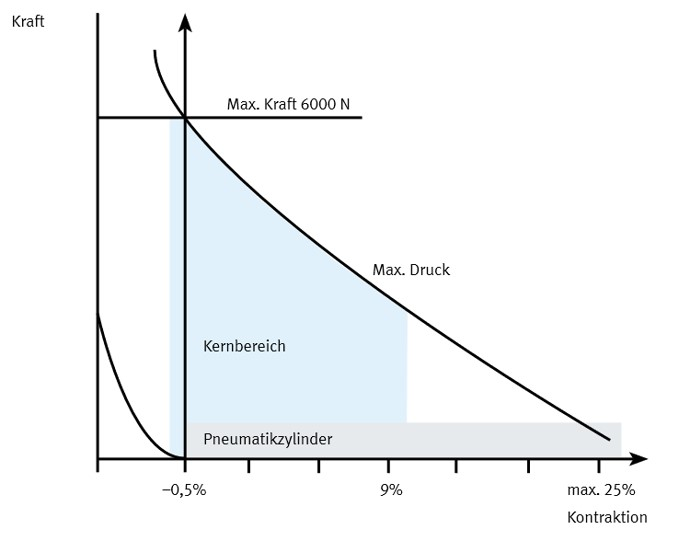
\includegraphics[width=.75\textwidth]{Abb/ArbeitsprofilDMSP.jpg}
			\caption{Arbeitsprofil eines künstlichen Muskels DMSP von Festo \cite{DMSP.specs}.}
			\label{fig:ArbeitsprofilDMSP}
		\end{figure}

		Wie auf \cref{fig:ArbeitsprofilDMSP} zusehen ist, liegt die maximal aufbringbare Kraft eines künstlichen Muskels deutlich über der eines Pneumatikzylinders.
		Außerdem skaliert seine Kraft mit dem Druck nahezu linear, in einem bestimmten Bereich, dies ist für die Anpassung auf verschiedene Spieler und Stöße beim Billard von großem Vorteil.

		\begin{figure}[h]
			\centering
			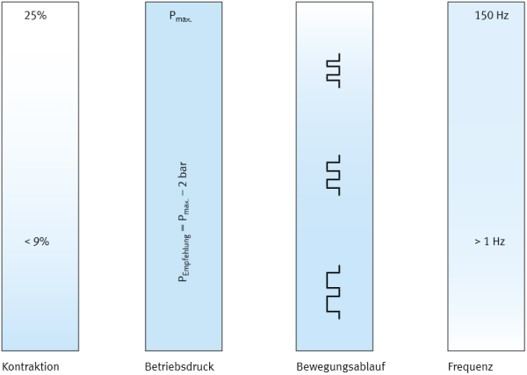
\includegraphics[width=.75\textwidth]{Abb/EigenschaftenkuenstlMuskel.jpg}
			\caption{Eigenschaften von künstlichen Muskeln \cite{DMSP.specs}.}
			\label{fig:EigenschaftenkuenstlMuskel}
		\end{figure}

		Wie in \cref{fig:EigenschaftenkuenstlMuskel} zu sehen gibt es aber auch einen entscheiden Nachteil, die Kraft, die der Muskel aufbringen kann, nimmt bei höherer Frequenz, also Geschwindigkeit des Stoßes, ab.
		Dies bedeutet, dass es unter Umständen schwierig sein kann, mit der Konstruktion schnelle und kraftvolle Stöße durchzuführen.

		\begin{figure}[h]
			\centering
			\includegraphics[width=\textwidth]{Abb/CAD/Renderings/sehnen_und_schelle.jpg}
			\caption[Gerenderte Darstellung der Sehnen und Sattelklemme]{Gerenderte Darstellung der Sehnen am Oberarm und der Klemme zur Fixierung der beiden Rohre.}%
			\label{fig:rendering sehnen und schellen}
		\end{figure}

		\begin{figure}[h]
			\centering
			\includegraphics[width=\textwidth]{Abb/CAD/Renderings/bizeps.jpg}
			\caption[Nahaufnahme des Bizeps bildenden pneumatischen Aktuators]{Nahaufnahme des Bizeps bildenden pneumatischen Aktuators.}%
			\label{fig:rendering bizeps}
		\end{figure}